\documentclass[12pt]{article}

\usepackage{sbc-template}

\usepackage{graphicx,url}

\usepackage{algorithm}
\usepackage{algpseudocode}

%\usepackage[brazil]{babel}   
\usepackage[latin1]{inputenc}  
     
\sloppy

\title{UKP5: a New Algorithm for the Unbounded Knapsack Problem}

\author{Henrique Becker \and Luciana S. Buriol}

\address{Instituto de Inform�tica -- Universidade Federal do Rio Grande do Sul
  (UFRGS)\\
  Caixa Postal 15.064 -- 91.501-970 -- Porto Alegre -- RS -- Brazil
  \email{\{hbecker,buriol\}@inf.ufrgs.br}
}

\begin{document} 

\maketitle

\begin{abstract}
In this extended abstract % resumo extendido -- short paper?
we present UKP5, an algorithm for solving the unbounded knapsack problem. 
UKP5 is based on dynamic programming, but implemented in a non traditional way: instead of looking backward for stored values of subproblems, it stores incremental lower bounds forward. 
%UKP5 uses sparsity, periodicity, and dominance for speeding up computation. 
UKP5 is considerably simpler than EDUK2, the state-of-the-art algorithm for solving the problem. 
%Moreover, it can be naturally implemented using the imperative paradigm, differently from EDUK2. 
We run UKP5 and EDUK2 on a benchmark of hard instances proposed by the authors of EDUK2. 
The benchmark is composed by 4540 instances, divided into five classes, with instances ranging from small to large inside each class. 
%Speedups were calculated for each class, and the overall speedup was calculated as the classes speedups average. 
The results reveal that UKP5 outperforms EDUK2, being 47 times faster on the average.
\end{abstract}

\section{Introduction}

\section{UKP5: The Proposed Algorithm}

\begin{algorithm}[!t]
\caption{UKP5 -- Computation of $opt$}\label{alg:ukp5}
\begin{algorithmic}[1]
\Procedure{UKP5}{$n, c, w, p, w_{min}, w_{max}$}
  \State \(g \gets\) array of \(c + w_{max}\) positions each one initialized with \(0\)\label{create_g}
  \State \(d \gets\) array of \(c + w_{max}\) positions each one initialized with \(n\)\label{create_d}
  
  \For{\(i \gets 1, n\)}\label{begin_trivial_bounds}\Comment{Stores one-item solutions}
    \If{\(g[w_i] < p_i\)}
      \State \(g[w_i] \gets p_i\)
      \State \(d[w_i] \gets i\)
    \EndIf
  \EndFor\label{end_trivial_bounds}

  \State \(opt \gets 0\)\label{init_opt}

  \For{\(y \gets w_{min}, c\)}\label{main_ext_loop_begin}\Comment{Can end early because of periodicity check}
    \If{\(g[y] \leq opt\)}\label{if_less_than_opt_begin}\Comment{Handles sparsity and pruning of dominated solutions}
    	\State \textbf{continue}\label{alg:continue}\Comment{Ends current iteration and begins the next}
    \EndIf\label{if_less_than_opt_end}
    
    \State \(opt \gets g[y]\)\label{update_opt}
    
    \For{\(i=1,d[y]\)}\label{main_inner_loop_begin}\Comment{Creates new solutions (never symmetric)}
      \If{\(g[y + w_i] < g[y] + p_i\)}\label{if_new_lower_bound_begin}
        \State \(g[y + w_i] \gets g[y] + p_i\)
        \State \(d[y + w_i] \gets i\)
%      \ElsIf{\(g[y + w_i] = g[y] + p_i \land i < d[y + w_i]\)}
%        \State \(d[y + w_i] \gets i\)
      \EndIf\label{if_new_lower_bound_end}
    \EndFor\label{main_inner_loop_end}
  \EndFor\label{main_ext_loop_end}
  \State \textbf{return} \(opt\)

%  \For{\(y \gets c-w_{min}+1, c\)}\label{get_y_opt_loop_begin}\Comment{Removal of dominated solutions}
%    \If{\(g[y] > opt\)}\label{last_loop_inner_if}
%      \State \(opt \gets g[y]\)
%      \State \(y_{opt} \gets y\)
%    \EndIf
%  \EndFor\label{get_y_opt_loop_end}
\EndProcedure
\end{algorithmic}
\end{algorithm}

\section{Computational Results and Analysis}

\begin{figure}[th]
  \label{fig:times}
  \centering
  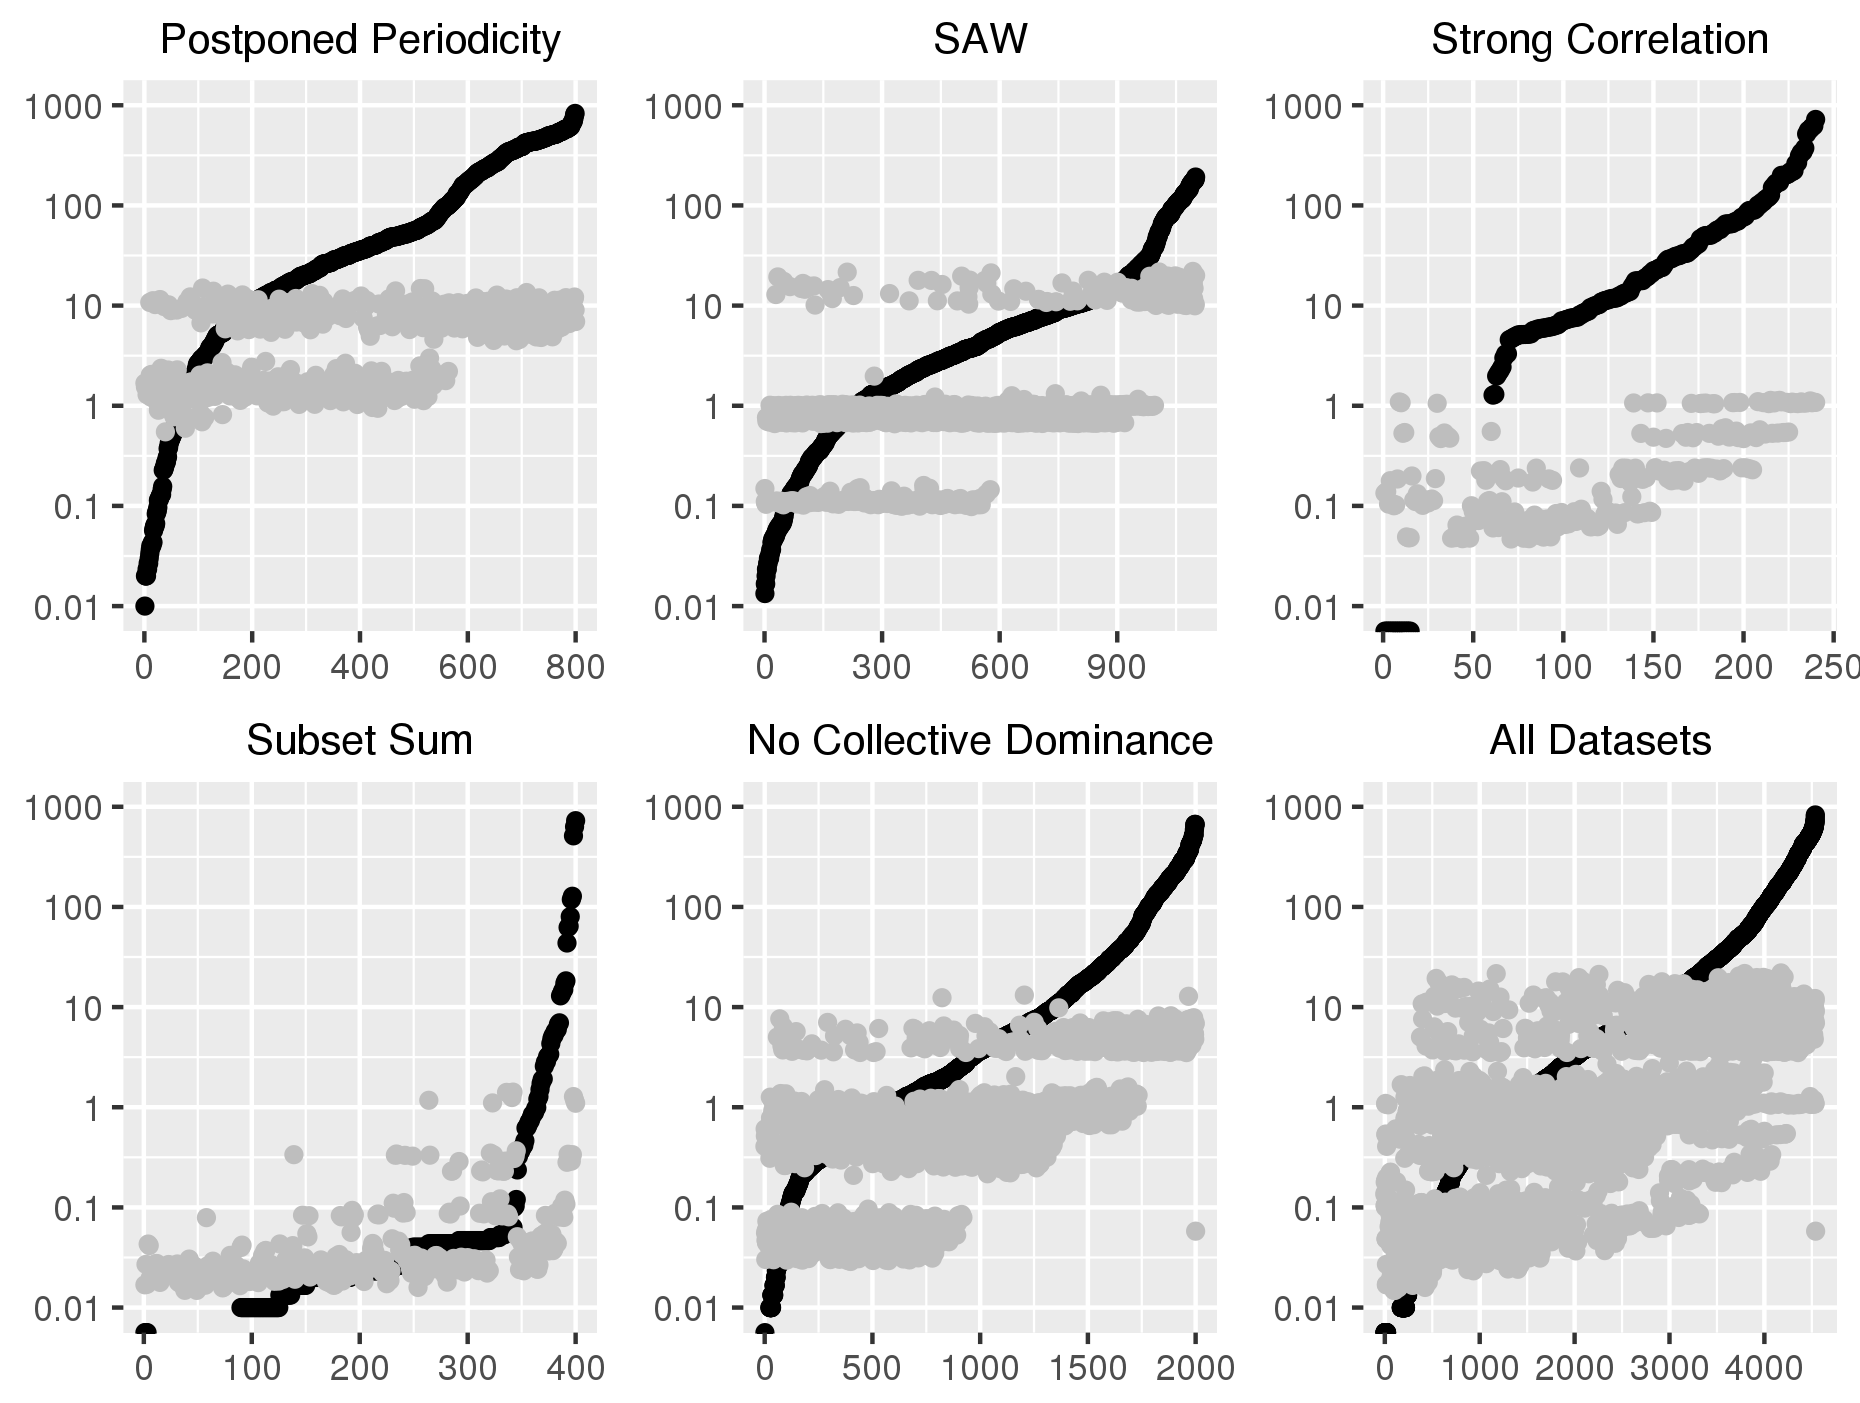
\includegraphics[width=\textwidth]{six_plots.png}
  \caption{The times used by UKP5 and PYAsUKP for each instance of each class. The black dots represent PYAsUKP times. The gray dots represent UKP5 times. The y axis is the time used to solve an UKP instance, in seconds. The x axis is the instance index when the instances are are sorted by the time PYAsUKP took to solve it. Note that the y axis is in logarithmic scale.}
\end{figure}

\section{Conclusion and Final Remarks}


\bibliographystyle{sbc}
\bibliography{sbc-template}

\end{document}
